\documentclass[../../main.tex]{subfiles}

\begin{figure}[ht]
    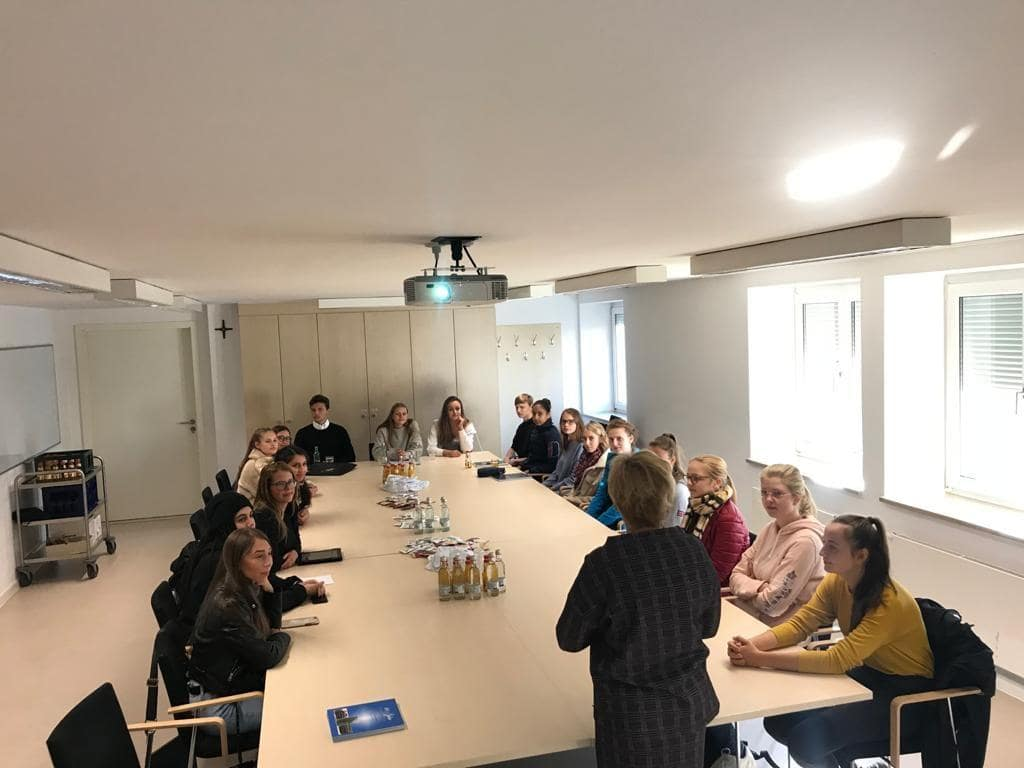
\includegraphics[width=\textwidth]{foto_hedwigsklinik_erstes_treffen.jpg}
\end{figure}

Am Montag, den 18. 11. kam unser P-Seminar Kurs mit den Mitarbeitern der Klinik St. Hedwig zusammen, um an der Hausführung teilzunehmen.

Zum Zweck der Informierung und Ideensammlung für alle Teilnehmer des P-Seminars wurden viele Bereiche der Klinik im Detail präsentiert. Die vorgestellten Räume und Abteilungen waren u. A. der MRT-Raum, der Schock-Raum und die Eingangshalle. Während die genannten Themen für die Zuständigen der Gerätegestaltung und des Positiven Zugangs relevant sind, ist für mein Thema das Patientenzimmer bedeutsam. Es sind durchaus gepflegte Zimmer, jedoch gibt es einige Gesichtspunkte, an denen man die Erfahrung beurteilen kann.

Zunächst lässt sich feststellen, dass nur beschränkt Wifi angeboten wird. ob es also ausreichend für Patienten verfügbar ist, werde ich nachgehen. Angenehmer wäre aber für jeden Anwesenden – einschließlich Eltern und Besucher – uneingeschränktes freies Wifi. Mit verlässlichem Internetzugang ist die Situation durchaus stressfreier.

Dazu kommt, dass für ein zwei-Betten-Zimmer nur ein Fernseher vorgesehen ist. Das kann zum Problem werden, wenn zwei untergebrachte Patienten unabhängig voneinander Spielen oder Fernsehen möchten. Um den ihnen diese Möglichkeit zu gewähren, ist es auch wichtig, Kopfhörer anzubieten.

In dieser Hinsicht gibt es aber bei der Umsetzung Probleme, die berücksichtigt werden müssen. Diese Problematik der Hygiene ist mir erst bei der Hausführung in Erscheinung getreten, als das Thema angesprochen wurde. Bei jeder zu verwirklichen Idee sind Einschränkungen wie diese nicht zu vernachlässigen, da die Gesundheit und Sicherheit des Patienten immer im Vordergrund stehen.

Mit den neu erworbenen Informationen aus der Hausführung werde ich einige Maßnahmen nehmen, um das Bestmögliche Ergebnis bei der Gestaltung meines Themas zu erzielen. In erster Linie werde ich Rücksicht auf Einschränkungen nehmen, und das Thema Realisierbar machen. Mein wichtigstes Anliegen ist es, die optimale Erfahrung für Patienten zu bieten, ohne die Gesundheit und Sicherheit zu opfern.

Trotz der umfassenden Hausführung fehlen mir noch einige Informationen, um meine Ideen umzusetzen. Da Free Wifi ein zentraler Teil der Erfahrung eines Klinikbesuchers ist, sowohl zur Unterhaltung und Kommunikation, als auch zur Freizeitbeschäftigung mit digitalen Spielen, möchte ich Fragen, ob untergebrachte Patienten einen Zugang erhalten, und, ob es Umsetzbar wäre, das Wifi für alle Besucher frei zu machen. Ein weiterer wichtiger Anhaltspunkt ist das verfügbare Budget. Das Endergebnis soll schließlich auch von den Kosten her realistisch sein. Außerdem interessiert mich, ob abgesehen von dem einen Fernseher pro Zimmer bereits andere wiederverwendbare Technik besteht, um Kosten zu reduzieren.
